\documentclass[12pt]{article}
\usepackage{amsmath}
\usepackage{amsfonts}
\usepackage{graphicx}
\DeclareGraphicsExtensions{.pdf,.png,.jpg}
\usepackage{algpseudocode}

\newtheorem{theorem}{Theorem}[section]
\newtheorem{lemma}[theorem]{Lemma}
\newtheorem{definition}[theorem]{Definition}


\title{Sampling in 2D}
\date{}
\begin{document}
  \maketitle
  
  Specify the 2D space $D \in \mathbb{R}^2$ to be a square without obstacles. Let $P = \{ p_1, p_2, ..., p_i, ... \}$ be a set of iso-cost contours where $\forall x \in p_i, clearance(x) = c_i$. \\
  
  For $x\in D$, we define $B_D(x)$ to be the largest closed disc centered at $x$ that is a subset of $D$, i.e., $B_D(x) = \overline{B}( x, \rho_{D}(x) )$, where $\overline{B}( x, \rho_{D}(x) )$ denotes the closed disc of radius $r \geq 0$, centered at $x$, and $\rho_{D}(x) = dist(x, \mathbb{R}^2 \setminus D)$ is the distance to the boundary for points inside $S$, and 0 for points outside $D$.
  
  The media axis $MA(D)$ of $S$ is defined to be the set of all points $x$ of $D$ whose $B_D(x)$ are maximal. $\cite{steven}$
  
  %$MA(D) = \{ x \in D | notexists y \in D$ $with$ $B_D(x) subsetneq B_D(y) \}$\\
  
  %Assume we are continuously sampling in the 2D space. $S_m = \{ B_D(x) | not \exists B_d(x) \in S_m with x' < x \wedge B_D(x') \subset B_D(x), \rho_D(x) \geq r_{min} \}$
  
  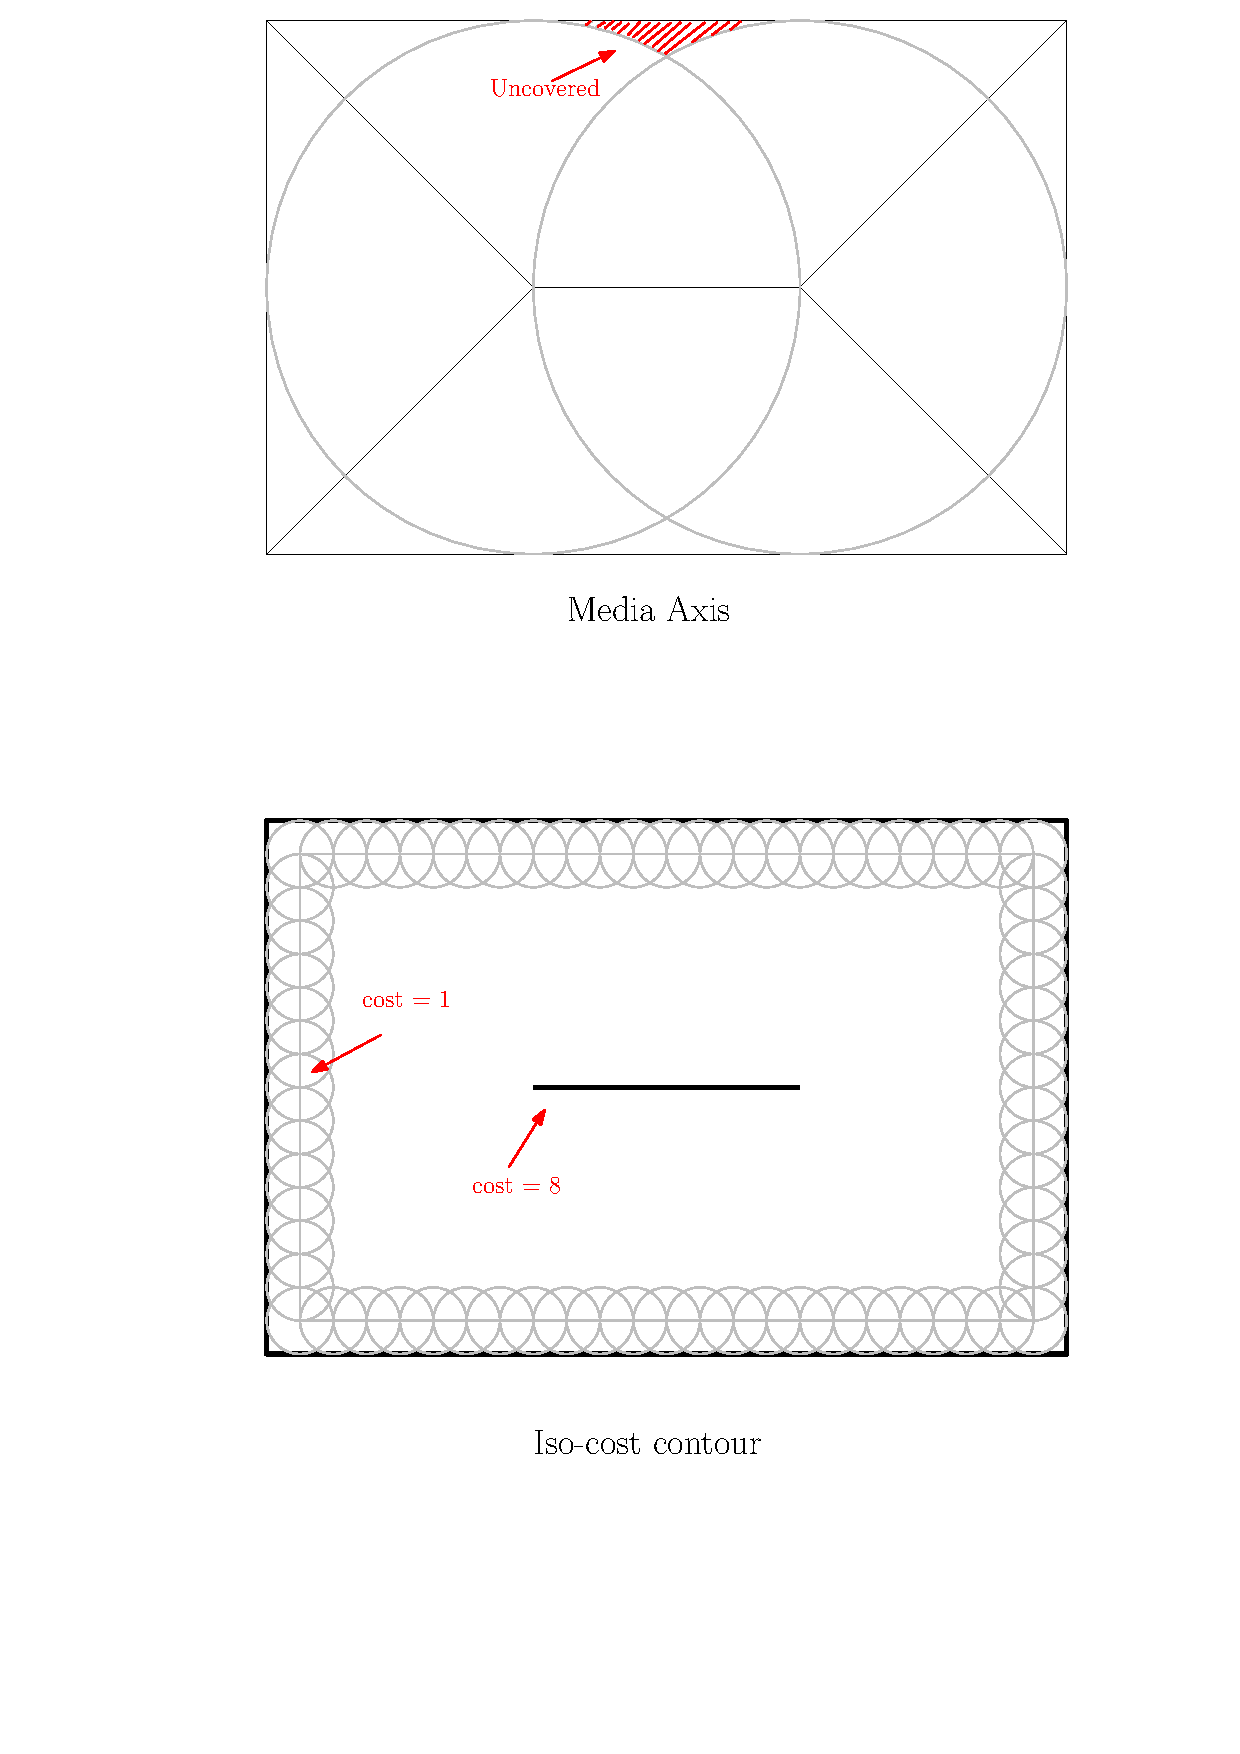
\includegraphics[scale=0.8]{./sampling2d/1.pdf}
  
  \section{Some Observations}
  \begin{enumerate}
  	\item Continuously sample all points $x \in MA(D)$ totally covers $D$.  $S_{c_{ma}} = \{B_D(x) | \forall x \in MA(D)\}$, $C(S_{c_{ma}}) = D$, where $C(S) = \cup_{\forall b \in S}$.
  	
  	\item Continuously sample all points $x \in P$ totally covers $D$, too.  $S_{c_{iso}} = \{B_D(x) | \forall x \in P\}$, $C(S_{c_{iso}}) = D$.
  	
  	\item Even if we can continuously sample in $MA(D)$, but restrict new balls to center outside existing ones, some areas near obstacles will be uncovered. 
    
    \item Use iso-cost contours to sample small balls can cover these left areas. Questions: How many contours do we need? What are the costs for these contours?
  	
  \end{enumerate}
  
  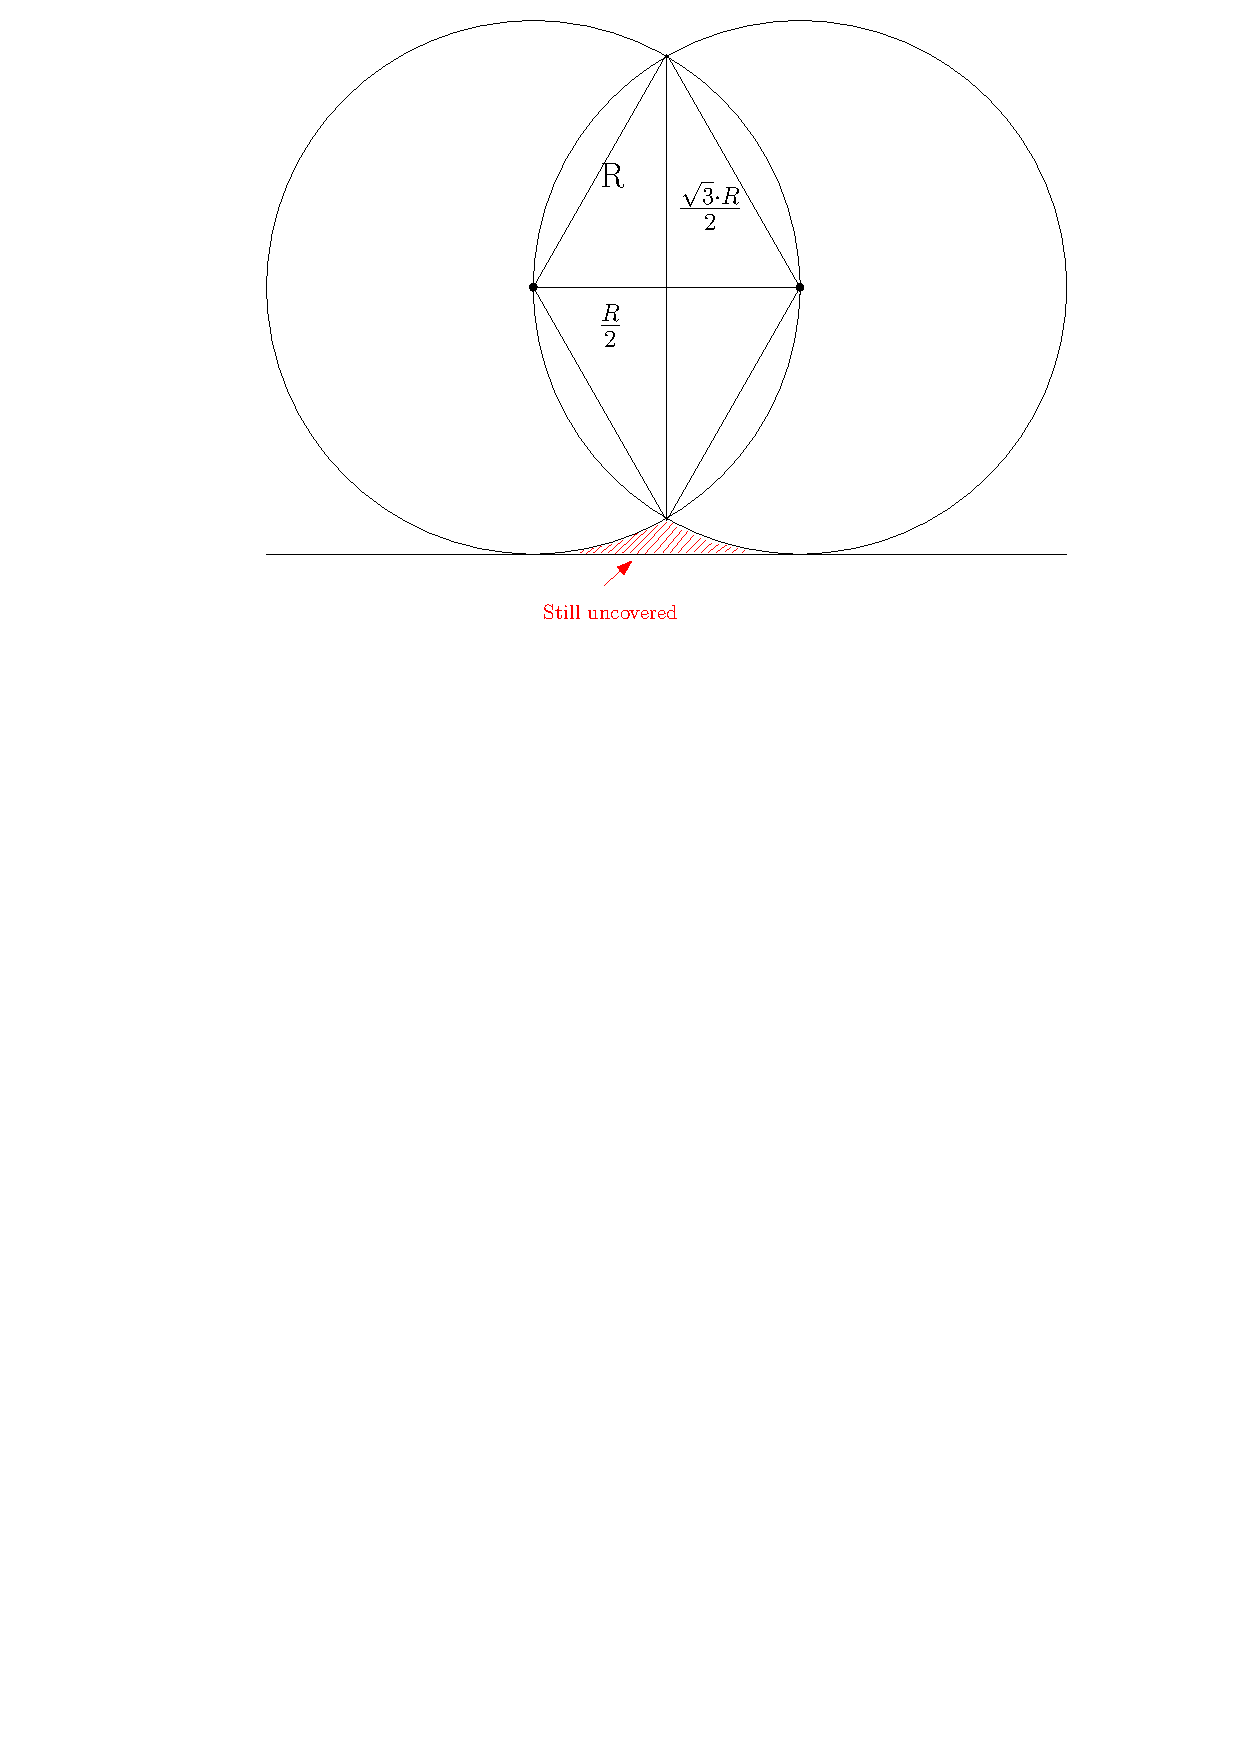
\includegraphics[scale=0.8]{./sampling2d/2discs.pdf}
  
  Assume a series of discs with the same radius $R$ and center on each other's boundary. Connect the centers, points within $\frac{\sqrt{3}R}{2}$ from the connecting line are guaranteed to be covered in the discs chain.\\
  
  If we want to cover all points in the left areas, assume the point farthest from obstacles has clearance $C_{max}$, we requires $(\frac{\sqrt{3}}{2} + 1) \cdot R = C_{max}$. $R = \frac{ 2\cdot C_{max} }{\sqrt{3}+2}$\\
  
  Now there are three possible situations: 
  
  1. $R = r_{min}$. 
  
  2. $R < r_{min}$.
  
  3. $R > r_{min}$.\\  
  
  If $R = r_{min}$, fine, just sample the contour with cost $c_i = r_{min}$.
  
  If $R < r_{min}$, still sample the contour with cost $c_i = r_{min}$.
  
  If $R > r_{min}$, sample the contour with cost $c_i = R$. Then repeat the process.
  
  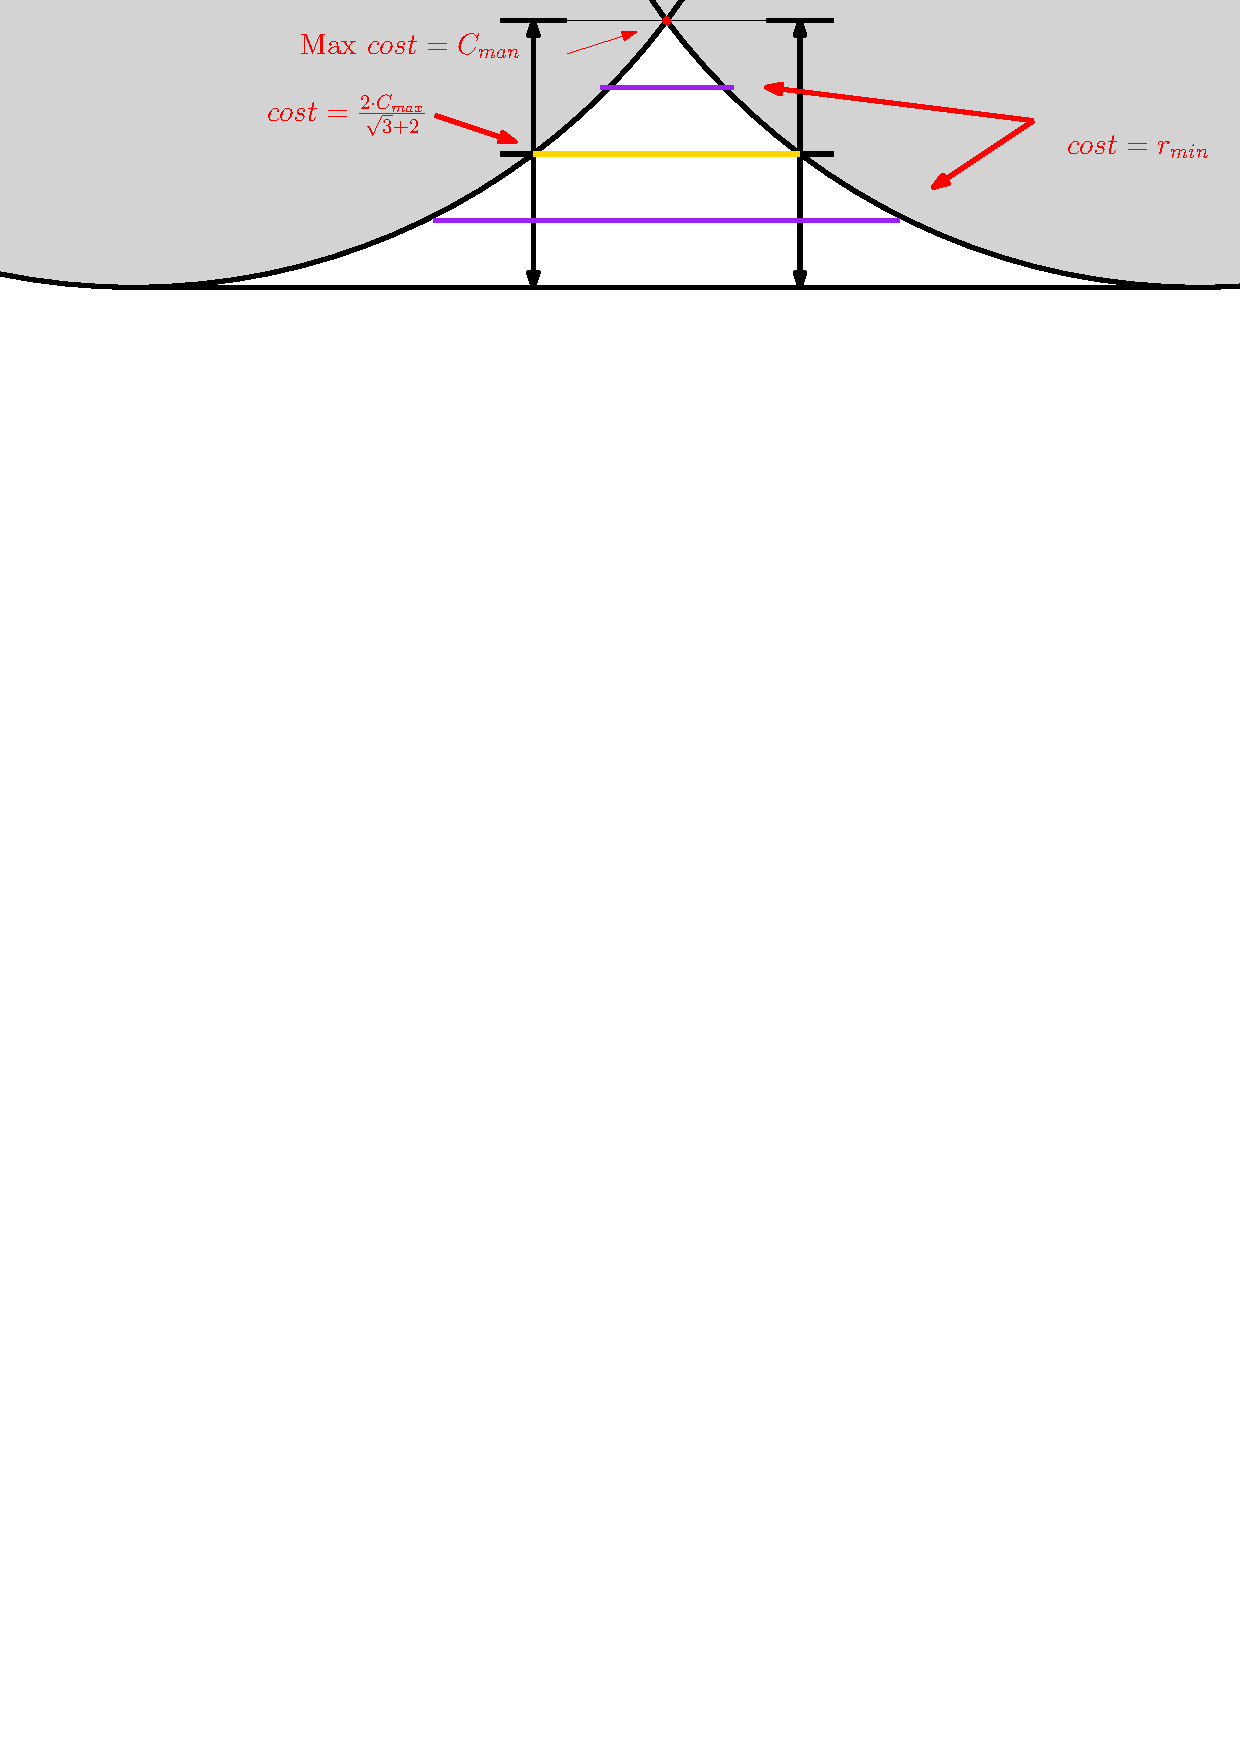
\includegraphics[scale=0.6]{./sampling2d/3.pdf}
  
  
  \section{Sampling on Media Axis} 
  
  In $\cite{steven}$, the author proposed an algorithm to sample on the media axis:\\
  
  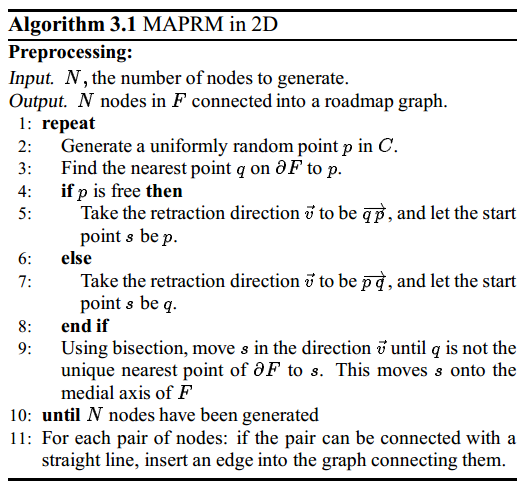
\includegraphics[scale=0.6]{./sampling2d/MAPRM.png}  
  
  By changing the terminal condition in line 9, we can sample discs with any radius. \\
    
  %\section{Growing the Obstacles}

        
  
  \begin{thebibliography}{1}

  \bibitem{steven} Steven A. Wilmarth, Nancy M. Amato, Peter F. Stiller. "MAPRM: A Probabilistic Roadmap Planner with Sampling on the Medial Axis of the Free Space", In Proc. IEEE Int. Conf. Robot. Autom. (ICRA), pp. 1024-1031, Detroit, MI, May 1999. Also, Technical Report, TR98-0022, Department of Computer Science and Engineering, Texas A \& M University, Nov 1998.

  \end{thebibliography}
  
\end{document}
  